\LARGE{Assignment 3:} \Large{Hall Effect Thruster}\\
\large{Space propulsion}\\
January 24, 2019
\begin{flushright}
\large{Álvaro Boix Candil}\\
\large{Carlos Molina Ordóñez}\\
\large{M. Nùria Partal Camps}\\
\end{flushright}

\section{Problem description}

The main objective of this project is the study of a Hall Effect Thruster,
specifically about the evolution of some parameters along its annular channel,
which will be analysed thanks to a one-dimensional model of it.
Xenon will be the propellant of the thruster
($\sigma_0 = 3.6 \cdot 10^{-20} m^2$, $m_i = 2.2\cdot 10^{-25} kg$, $V_i = 12.1 V$,
$E_i = eV_i$),
the channel width is $H = 15 mm$ and the given mean radius is $r_m = 50mm$. The
channel length will be considered about $L = 20 mm$. It must be assumed that at
the inlet $\Gamma_{i,B} / \Gamma_m = 0.01$ and the problem will be developed using non-dimensional
variables.

Using the given data and from formulas extracted from theory lessons, the following
parameters have been determined: $T_{eB}$, $v_{iB}$, $n_{eB}$, $n_{iB}$, $\Gamma_{eB}$,
$v_{eB}$, $p_{eB}$, $\Gamma_nB$, $n_{nB}$, $n_B$, $v_{exB}$, $\nu_{enB}$, $\omega_c$,
$\nu_{eB}$, $\nu_{iB}$, and $\phi$. Here, the sub-index B indicates the value of
a parameter at the initial position.

Joining these data and the adimensionalization factors identified by a star,
the previous adimensionalized parameters have been obtained.

Once this is done, the system of differential equations has been solved:

\begin{equation}
	\small
	\left[\frac{5}{3}T_e-v_i^2\right]\frac{dv_{i}}{dx} = \frac{5}{3}\frac{m_e}{m_i}\left(v_i-\frac{\Gamma_d}{n_e}\right)\nu_e v_i + \nu_i\left(\frac{5}{3}T_e + v_i(v_i-c_n)-\frac{v_i}{v_ex}\left[\frac{2}{3}E_i'+\frac{5}{3}T_e\right]\right)
\end{equation}
\begin{equation}
	\small
	\left[\frac{5}{3}T_e-v_i^2\right]\frac{d n_{e}}{dx} = -\frac{5}{3}\frac{m_e}{m_i}n_e v_ex\nu_e - n_e\nu_i\left((2v_i-c_n)-\left[\frac{2}{3}E_i'+\frac{5}{3}T_e\right]\frac{1}{v_ex}\right)
\end{equation}
\begin{equation}
	\small
	\left[\frac{5}{3}T_e-v_i^2\right]\frac{d T_{e}}{dx} = -\frac{2}{3}v_i^2\frac{m_e}{m_i}v_ex\nu_e-\nu_i\left(\frac{2}{3}T_e(2v_i-c_n)-\left[\frac{v_i^2-T_e}{v_ex}\right]\left[\frac{2}{3}E_i'+\frac{5}{3}T_e\right]\right)
\end{equation}
\begin{equation}
	\small
	\left[\frac{5}{3}T_e-v_i^2\right]\frac{d{\phi}}{dx} = -\frac{5}{3}\frac{m_e}{m_i}v_ex\nu_e v_i^2-\nu_i\left(\frac{5}{3}T_e(2v_i-c_n)-\frac{v_i^2}{v_ex}\left[\frac{2}{3}E_i'+\frac{5}{3}T_e\right]\right)
\end{equation}

In order to solve this system, a Matlab function that implements \texttt{ode45}
has been used.

Then it has been calculated the thrust with:

\begin{equation}
	\frac{F}{A} = m_i(\Gamma_i \nu_i)_E + (p_e)_E
\end{equation}
, where $p_e = n_e kT_e$ is the electron pressure, and the subscript E refers to
the end section of the thruster, upon reaching the sonic speed, and A is the
cross sectional area $A = 2\pi r m H$

And finally, also the efficiency has been obtained by computing:

\begin{equation}
	\eta_p = \frac{\dot{m}c^2}{2P} = \frac{F^2/\dot{m}}{2P}
\end{equation}

where the input power is calculated as:

\begin{equation}
	P = I V = e \Gamma_d A
\end{equation}

\section{Results}

The next plot in figure \ref{fig:phi} shows the results for the potential $\phi$
distribution along x axis.
It can be appreciated that, for lower values of ratio $kT_e/E_i$ the value of the
voltage is more stable. In the case of 0.2 ratio, the value of the voltage in
average is the double of the one obtained for 0.1. That could reveal a possible
linear relation between the temperature and the voltage obtained.

The graph for $\Gamma$ is shown in figure \ref{fig:gamma}.
Observing the distribution of $\Gamma_i$, which represents the ions mass flow,
it is observed that it's only positive for positions at the end of the acceleration
chamber, that cold mean that some of the ions that came from the fuel inlet remain trapped
in the beginning area until they enter in the area of ionization, where they start
accelerated, so they gain positive x velocity. Also it's observed that for larger
temperature-electric field ratios, the maximum ion mass flow is smaller and the
length of the acceleration chamber should also be shorter.

As can be seen from Figure \ref{fig:ne}, comparing for the different values of
$kT_e/E_i$, the number of electrons increases as the Temperature decreases since
the electron velocity, and thus the electron collisions, increases. Analogously
to Figure \ref{fig:enumber}, the temperature increases as the $kT_e/E_i$ ratio
increases. On the other hand, the increase on $kT_e/E_i$ ratio, and thus on temperature,
produces an increase in the Mach number (Figure \ref{fig:mach}), since the velocity
is dependent on this ratio.

And finally, the results for the calculated Thrust and Efficiency for each ratio
considered are shown in the next table \ref{tab:results}. This results also agree with
the ones observed in some of the previous plots. When the ratio decreases, the
thrust increases, and also the efficiency, because for example, the number of
electrons increases and the mass flow of ions at the end of the acceleration chamber,
which is also larger.

\begin{table}[]
\centering
\begin{tabular}{ccc}
$kT_e/E_i$ & Thrust (N) & Efficiency \\ \hline
0.1000 & 0.3190 & 0.5120 \\ \hline
0.1500 & 0.0545 & 0.0717 \\ \hline
0.2000 & 0.0239 & 0.0306 \\ \hline
\end{tabular}
\caption{Thurst and efficiency values for each ratio considered}
\label{tab:results}
\end{table}


\begin{figure}[h!]
	\centering
	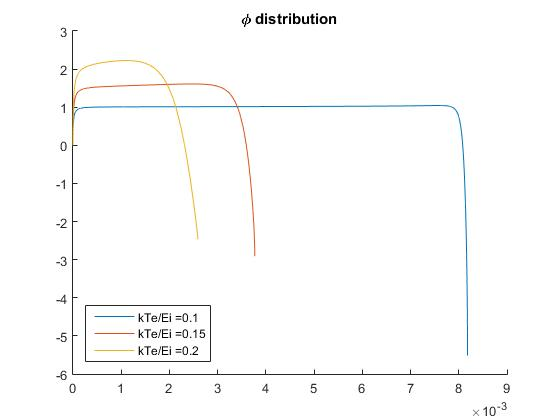
\includegraphics[width=0.8\textwidth]{img/Phi.jpg}
	\caption{$\phi$ potential distribution along x axis}
	\label{fig:phi}
\end{figure}

\begin{figure}[h!]
	\centering
	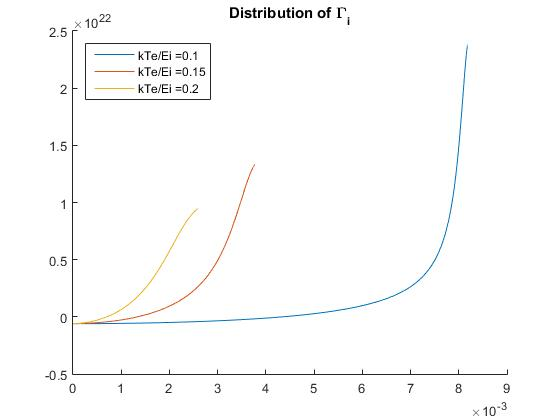
\includegraphics[width=0.8\textwidth]{img/Gamma_i.jpg}
	\caption{$\Gamma$ distribution along x axis}
	\label{fig:gamma}
\end{figure}

\begin{figure}[h!]
	\centering
	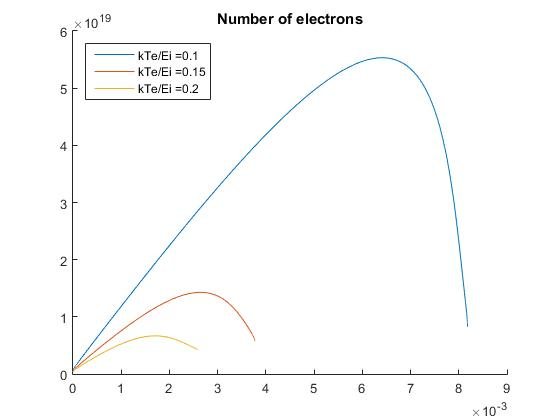
\includegraphics[width=0.8\textwidth]{img/Electrons_number.jpg}
	\caption{Electron density $(n_e)$ distribution along x axis}
	\label{fig:ne}
\end{figure}

\begin{figure}[h!]
	\centering
	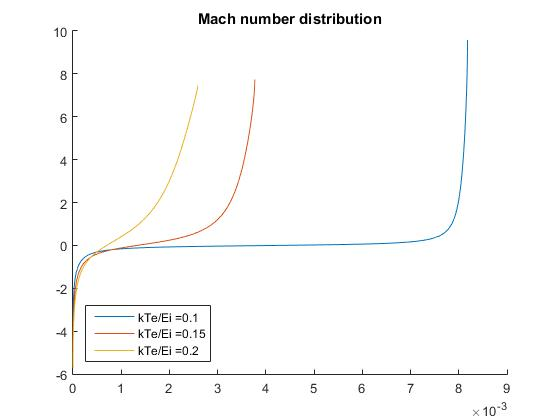
\includegraphics[width=0.8\textwidth]{img/Mach.jpg}
	\caption{Mach number distribution along x axis}
	\label{fig:mach}
\end{figure}

\begin{figure}[h!]
	\centering
	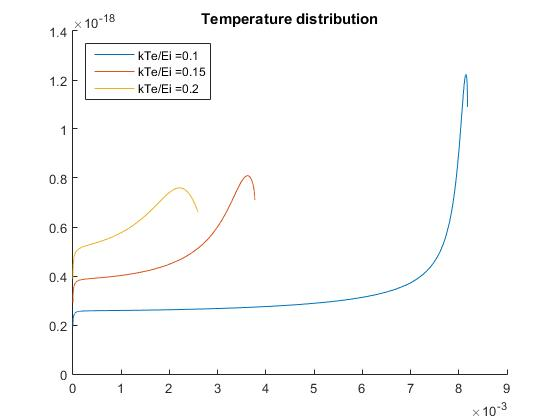
\includegraphics[width=0.8\textwidth]{img/Temperature.jpg}
	\caption{Temperature distribution along x axis}
	\label{fig:temp}
\end{figure}
